% Shared layout of the IPTV quick start guides (one file per language:
% IPTV-Quick-Start.tex, IPTV-Quick-Start-it.tex, ...). Each sets, before
% % Shared layout of the IPTV quick start guides (one file per language:
% IPTV-Quick-Start.tex, IPTV-Quick-Start-it.tex, ...). Each sets, before
% % Shared layout of the IPTV quick start guides (one file per language:
% IPTV-Quick-Start.tex, IPTV-Quick-Start-it.tex, ...). Each sets, before
% % Shared layout of the IPTV quick start guides (one file per language:
% IPTV-Quick-Start.tex, IPTV-Quick-Start-it.tex, ...). Each sets, before
% \input{preamble}:
%   \GuideLang   babel language (english, italian, spanish, french, ngerman, portuguese)
%   \GuideTitle  the guide's title, used on the cover, in headers and the PDF
%   \TipLabel    the word that starts a tip box ("Tip.")
% Build any of them with pdflatex, twice (for the table of contents).
\documentclass[11pt,a4paper]{article}

\usepackage[T1]{fontenc}
\usepackage[utf8]{inputenc}
% shorthands=off: no language-specific active characters (they would clash
% with tables and addresses); only hyphenation and "Contents" etc. change.
\usepackage[shorthands=off,\GuideLang]{babel}
\usepackage{lmodern}
\usepackage[scaled=0.92]{helvet}
\renewcommand{\familydefault}{\sfdefault}
\usepackage[margin=2.2cm,headheight=14pt]{geometry}
\usepackage{graphicx}
\usepackage[table]{xcolor}
\usepackage{booktabs}
\usepackage{tabularx}
\usepackage{xltabular}
\usepackage{enumitem}
\usepackage{titlesec}
\usepackage{fancyhdr}
\usepackage{pifont}
\usepackage{amssymb}
\usepackage[hidelinks]{hyperref}

\newcommand{\version}{0.12}
\definecolor{accent}{HTML}{1E6FD9}
\definecolor{dim}{HTML}{5F6673}
\definecolor{notebg}{HTML}{EEF4FC}
\definecolor{warnbg}{HTML}{FFF6E0}
\definecolor{tvred}{HTML}{D32F2F}
\definecolor{tvgreen}{HTML}{2E7D32}
\definecolor{tvyellow}{HTML}{C9A400}
\definecolor{tvblue}{HTML}{1565C0}

\hypersetup{pdftitle={IPTV -- \GuideTitle}, pdfauthor={IPTV project}}
\setlist{itemsep=2pt, topsep=4pt}
\setlength{\parindent}{0pt}
\setlength{\parskip}{6pt}
\renewcommand{\arraystretch}{1.25}

\titleformat{\section}{\Large\bfseries\color{accent}}{\thesection}{0.6em}{}
\titleformat{\subsection}{\large\bfseries}{\thesubsection}{0.6em}{}
\titlespacing*{\section}{0pt}{14pt}{6pt}
\titlespacing*{\subsection}{0pt}{10pt}{4pt}

\pagestyle{fancy}
\fancyhf{}
\fancyhead[L]{\small\color{dim}IPTV -- \GuideTitle}
\fancyhead[R]{\small\color{dim}github.com/vickdini/iptv}
\fancyfoot[C]{\small\color{dim}\thepage}
\renewcommand{\headrulewidth}{0.4pt}
\renewcommand{\sectionmark}[1]{\markboth{#1}{}}

% A key or button on a keyboard / remote.
\newcommand{\key}[1]{{\setlength{\fboxsep}{1.5pt}\fbox{\footnotesize\vphantom{Ay}#1}}}
% A coloured remote button.
\newcommand{\colorkey}[2]{\textcolor{#1}{\ding{108}}\,\textbf{#2}}
% Shaded boxes for tips and notes.
\newcommand{\tip}[1]{\par\noindent\colorbox{notebg}{\parbox{\dimexpr\linewidth-2\fboxsep}{\small\textbf{\TipLabel} #1}}\par}
\newcommand{\note}[1]{\par\noindent\colorbox{warnbg}{\parbox{\dimexpr\linewidth-2\fboxsep}{\small #1}}\par}
\newcommand{\menu}[1]{\textit{#1}}
\newcommand{\download}{\url{https://github.com/vickdini/iptv/releases/latest}}
% Key tables: \rowcolors{2}{gray!8}{white} then
% \begin{xltabular}{\linewidth}{@{}KX@{}} \keyshead{Key}{What it does} ... \bottomrule
\newcolumntype{K}{>{\raggedright\arraybackslash}p{5.4cm}}
\newcommand{\keyshead}[2]{\toprule \textbf{#1} & \textbf{#2} \\ \midrule}

% The cover: #1 subtitle, #2 "Version".
\newcommand{\cover}[2]{%
\begin{titlepage}
  \centering
  \vspace*{0.5cm}
  {\fontsize{40}{48}\selectfont\bfseries\color{accent} IPTV\par}
  \vspace{0.3cm}
  {\LARGE \GuideTitle\par}
  \vspace{0.3cm}
  {\large\color{dim} #1\par}
  \vspace{1cm}
  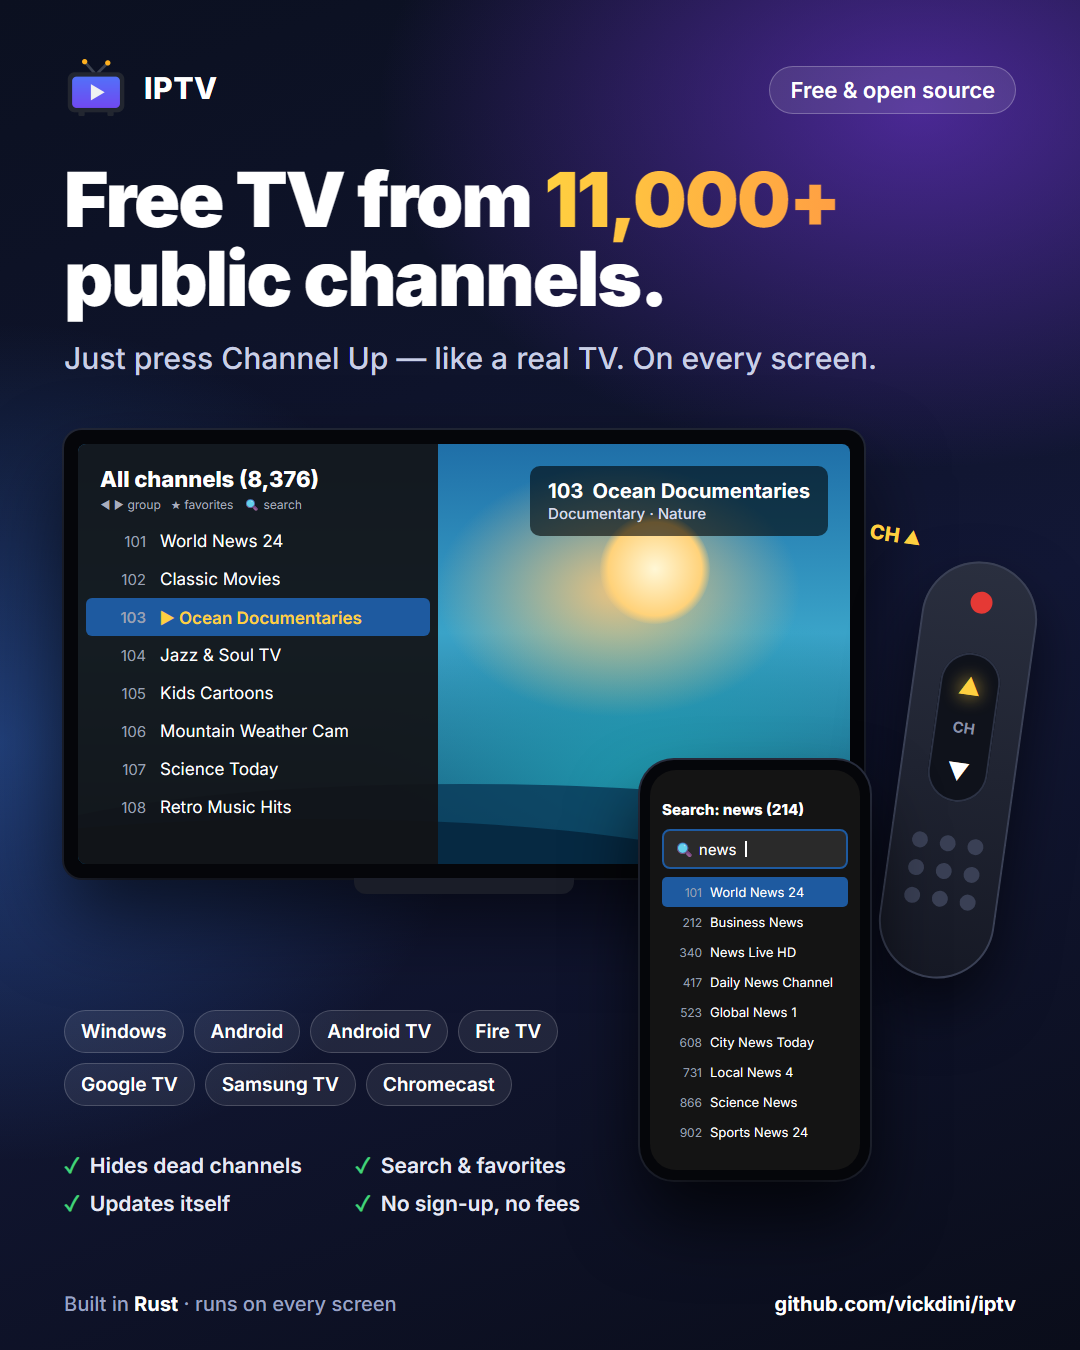
\includegraphics[width=0.52\textwidth]{../images/iptv-overview.png}\par
  \vfill
  {\large Windows \textbullet{} macOS \textbullet{} Linux \textbullet{} Android
   \textbullet{} Android TV \& Fire TV \textbullet{} Chromecast \textbullet{} Samsung TV\par}
  \vspace{0.5cm}
  {\color{dim} #2 \version{} \textbullet{} \url{https://github.com/vickdini/iptv}\par}
\end{titlepage}
\tableofcontents
\thispagestyle{fancy}}
:
%   \GuideLang   babel language (english, italian, spanish, french, ngerman, portuguese)
%   \GuideTitle  the guide's title, used on the cover, in headers and the PDF
%   \TipLabel    the word that starts a tip box ("Tip.")
% Build any of them with pdflatex, twice (for the table of contents).
\documentclass[11pt,a4paper]{article}

\usepackage[T1]{fontenc}
\usepackage[utf8]{inputenc}
% shorthands=off: no language-specific active characters (they would clash
% with tables and addresses); only hyphenation and "Contents" etc. change.
\usepackage[shorthands=off,\GuideLang]{babel}
\usepackage{lmodern}
\usepackage[scaled=0.92]{helvet}
\renewcommand{\familydefault}{\sfdefault}
\usepackage[margin=2.2cm,headheight=14pt]{geometry}
\usepackage{graphicx}
\usepackage[table]{xcolor}
\usepackage{booktabs}
\usepackage{tabularx}
\usepackage{xltabular}
\usepackage{enumitem}
\usepackage{titlesec}
\usepackage{fancyhdr}
\usepackage{pifont}
\usepackage{amssymb}
\usepackage[hidelinks]{hyperref}

\newcommand{\version}{0.12}
\definecolor{accent}{HTML}{1E6FD9}
\definecolor{dim}{HTML}{5F6673}
\definecolor{notebg}{HTML}{EEF4FC}
\definecolor{warnbg}{HTML}{FFF6E0}
\definecolor{tvred}{HTML}{D32F2F}
\definecolor{tvgreen}{HTML}{2E7D32}
\definecolor{tvyellow}{HTML}{C9A400}
\definecolor{tvblue}{HTML}{1565C0}

\hypersetup{pdftitle={IPTV -- \GuideTitle}, pdfauthor={IPTV project}}
\setlist{itemsep=2pt, topsep=4pt}
\setlength{\parindent}{0pt}
\setlength{\parskip}{6pt}
\renewcommand{\arraystretch}{1.25}

\titleformat{\section}{\Large\bfseries\color{accent}}{\thesection}{0.6em}{}
\titleformat{\subsection}{\large\bfseries}{\thesubsection}{0.6em}{}
\titlespacing*{\section}{0pt}{14pt}{6pt}
\titlespacing*{\subsection}{0pt}{10pt}{4pt}

\pagestyle{fancy}
\fancyhf{}
\fancyhead[L]{\small\color{dim}IPTV -- \GuideTitle}
\fancyhead[R]{\small\color{dim}github.com/vickdini/iptv}
\fancyfoot[C]{\small\color{dim}\thepage}
\renewcommand{\headrulewidth}{0.4pt}
\renewcommand{\sectionmark}[1]{\markboth{#1}{}}

% A key or button on a keyboard / remote.
\newcommand{\key}[1]{{\setlength{\fboxsep}{1.5pt}\fbox{\footnotesize\vphantom{Ay}#1}}}
% A coloured remote button.
\newcommand{\colorkey}[2]{\textcolor{#1}{\ding{108}}\,\textbf{#2}}
% Shaded boxes for tips and notes.
\newcommand{\tip}[1]{\par\noindent\colorbox{notebg}{\parbox{\dimexpr\linewidth-2\fboxsep}{\small\textbf{\TipLabel} #1}}\par}
\newcommand{\note}[1]{\par\noindent\colorbox{warnbg}{\parbox{\dimexpr\linewidth-2\fboxsep}{\small #1}}\par}
\newcommand{\menu}[1]{\textit{#1}}
\newcommand{\download}{\url{https://github.com/vickdini/iptv/releases/latest}}
% Key tables: \rowcolors{2}{gray!8}{white} then
% \begin{xltabular}{\linewidth}{@{}KX@{}} \keyshead{Key}{What it does} ... \bottomrule
\newcolumntype{K}{>{\raggedright\arraybackslash}p{5.4cm}}
\newcommand{\keyshead}[2]{\toprule \textbf{#1} & \textbf{#2} \\ \midrule}

% The cover: #1 subtitle, #2 "Version".
\newcommand{\cover}[2]{%
\begin{titlepage}
  \centering
  \vspace*{0.5cm}
  {\fontsize{40}{48}\selectfont\bfseries\color{accent} IPTV\par}
  \vspace{0.3cm}
  {\LARGE \GuideTitle\par}
  \vspace{0.3cm}
  {\large\color{dim} #1\par}
  \vspace{1cm}
  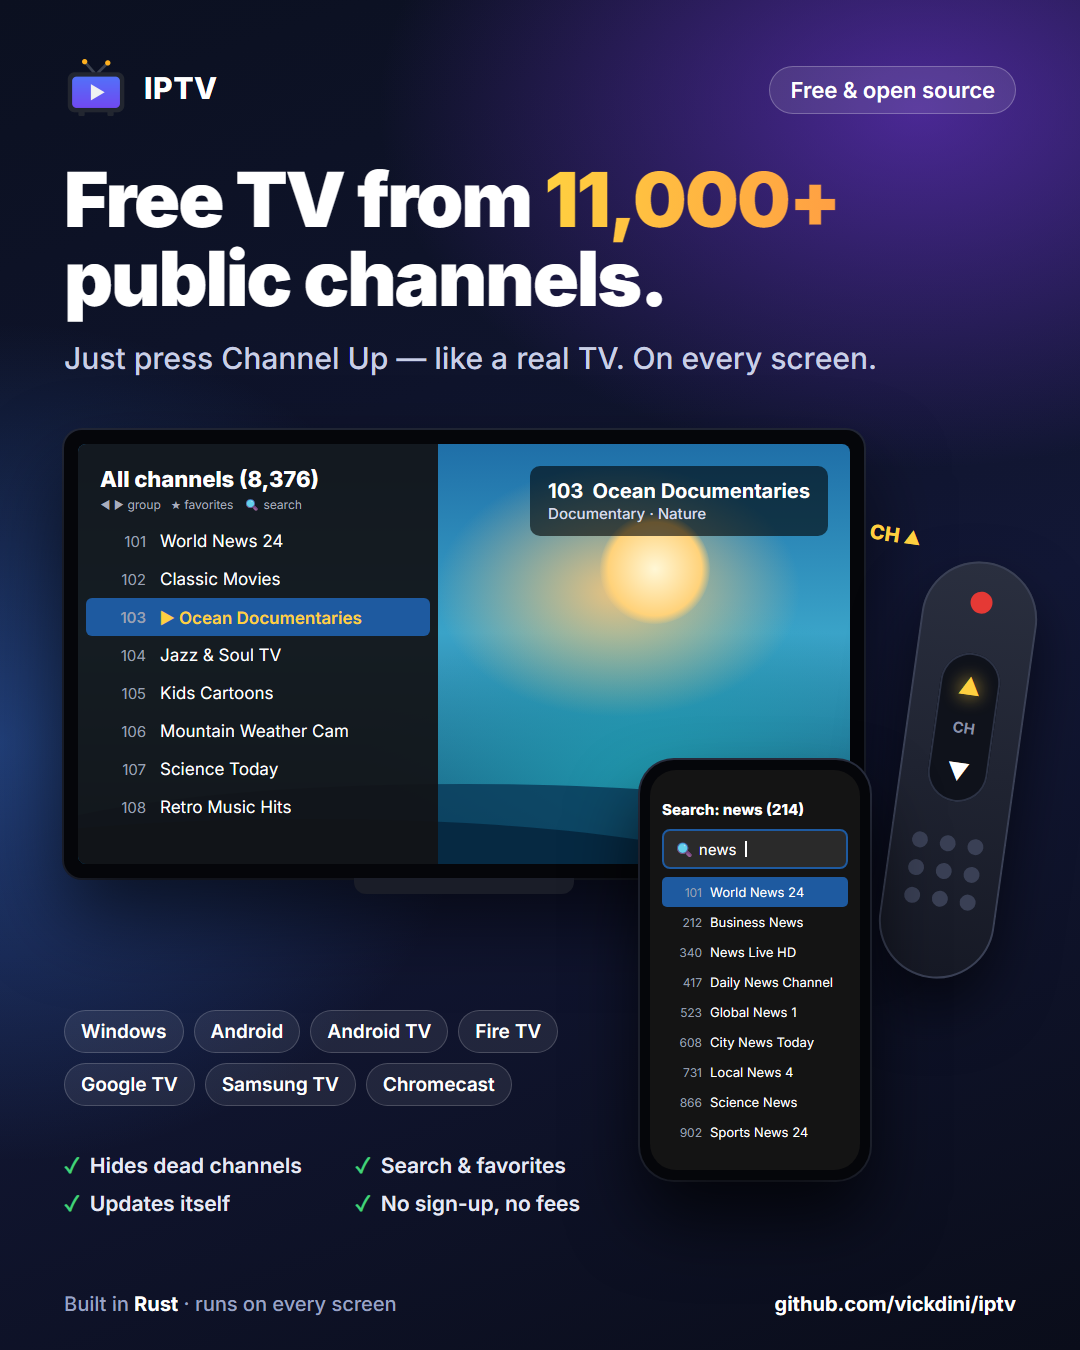
\includegraphics[width=0.52\textwidth]{../images/iptv-overview.png}\par
  \vfill
  {\large Windows \textbullet{} macOS \textbullet{} Linux \textbullet{} Android
   \textbullet{} Android TV \& Fire TV \textbullet{} Chromecast \textbullet{} Samsung TV\par}
  \vspace{0.5cm}
  {\color{dim} #2 \version{} \textbullet{} \url{https://github.com/vickdini/iptv}\par}
\end{titlepage}
\tableofcontents
\thispagestyle{fancy}}
:
%   \GuideLang   babel language (english, italian, spanish, french, ngerman, portuguese)
%   \GuideTitle  the guide's title, used on the cover, in headers and the PDF
%   \TipLabel    the word that starts a tip box ("Tip.")
% Build any of them with pdflatex, twice (for the table of contents).
\documentclass[11pt,a4paper]{article}

\usepackage[T1]{fontenc}
\usepackage[utf8]{inputenc}
% shorthands=off: no language-specific active characters (they would clash
% with tables and addresses); only hyphenation and "Contents" etc. change.
\usepackage[shorthands=off,\GuideLang]{babel}
\usepackage{lmodern}
\usepackage[scaled=0.92]{helvet}
\renewcommand{\familydefault}{\sfdefault}
\usepackage[margin=2.2cm,headheight=14pt]{geometry}
\usepackage{graphicx}
\usepackage[table]{xcolor}
\usepackage{booktabs}
\usepackage{tabularx}
\usepackage{xltabular}
\usepackage{enumitem}
\usepackage{titlesec}
\usepackage{fancyhdr}
\usepackage{pifont}
\usepackage{amssymb}
\usepackage[hidelinks]{hyperref}

\newcommand{\version}{0.12}
\definecolor{accent}{HTML}{1E6FD9}
\definecolor{dim}{HTML}{5F6673}
\definecolor{notebg}{HTML}{EEF4FC}
\definecolor{warnbg}{HTML}{FFF6E0}
\definecolor{tvred}{HTML}{D32F2F}
\definecolor{tvgreen}{HTML}{2E7D32}
\definecolor{tvyellow}{HTML}{C9A400}
\definecolor{tvblue}{HTML}{1565C0}

\hypersetup{pdftitle={IPTV -- \GuideTitle}, pdfauthor={IPTV project}}
\setlist{itemsep=2pt, topsep=4pt}
\setlength{\parindent}{0pt}
\setlength{\parskip}{6pt}
\renewcommand{\arraystretch}{1.25}

\titleformat{\section}{\Large\bfseries\color{accent}}{\thesection}{0.6em}{}
\titleformat{\subsection}{\large\bfseries}{\thesubsection}{0.6em}{}
\titlespacing*{\section}{0pt}{14pt}{6pt}
\titlespacing*{\subsection}{0pt}{10pt}{4pt}

\pagestyle{fancy}
\fancyhf{}
\fancyhead[L]{\small\color{dim}IPTV -- \GuideTitle}
\fancyhead[R]{\small\color{dim}github.com/vickdini/iptv}
\fancyfoot[C]{\small\color{dim}\thepage}
\renewcommand{\headrulewidth}{0.4pt}
\renewcommand{\sectionmark}[1]{\markboth{#1}{}}

% A key or button on a keyboard / remote.
\newcommand{\key}[1]{{\setlength{\fboxsep}{1.5pt}\fbox{\footnotesize\vphantom{Ay}#1}}}
% A coloured remote button.
\newcommand{\colorkey}[2]{\textcolor{#1}{\ding{108}}\,\textbf{#2}}
% Shaded boxes for tips and notes.
\newcommand{\tip}[1]{\par\noindent\colorbox{notebg}{\parbox{\dimexpr\linewidth-2\fboxsep}{\small\textbf{\TipLabel} #1}}\par}
\newcommand{\note}[1]{\par\noindent\colorbox{warnbg}{\parbox{\dimexpr\linewidth-2\fboxsep}{\small #1}}\par}
\newcommand{\menu}[1]{\textit{#1}}
\newcommand{\download}{\url{https://github.com/vickdini/iptv/releases/latest}}
% Key tables: \rowcolors{2}{gray!8}{white} then
% \begin{xltabular}{\linewidth}{@{}KX@{}} \keyshead{Key}{What it does} ... \bottomrule
\newcolumntype{K}{>{\raggedright\arraybackslash}p{5.4cm}}
\newcommand{\keyshead}[2]{\toprule \textbf{#1} & \textbf{#2} \\ \midrule}

% The cover: #1 subtitle, #2 "Version".
\newcommand{\cover}[2]{%
\begin{titlepage}
  \centering
  \vspace*{0.5cm}
  {\fontsize{40}{48}\selectfont\bfseries\color{accent} IPTV\par}
  \vspace{0.3cm}
  {\LARGE \GuideTitle\par}
  \vspace{0.3cm}
  {\large\color{dim} #1\par}
  \vspace{1cm}
  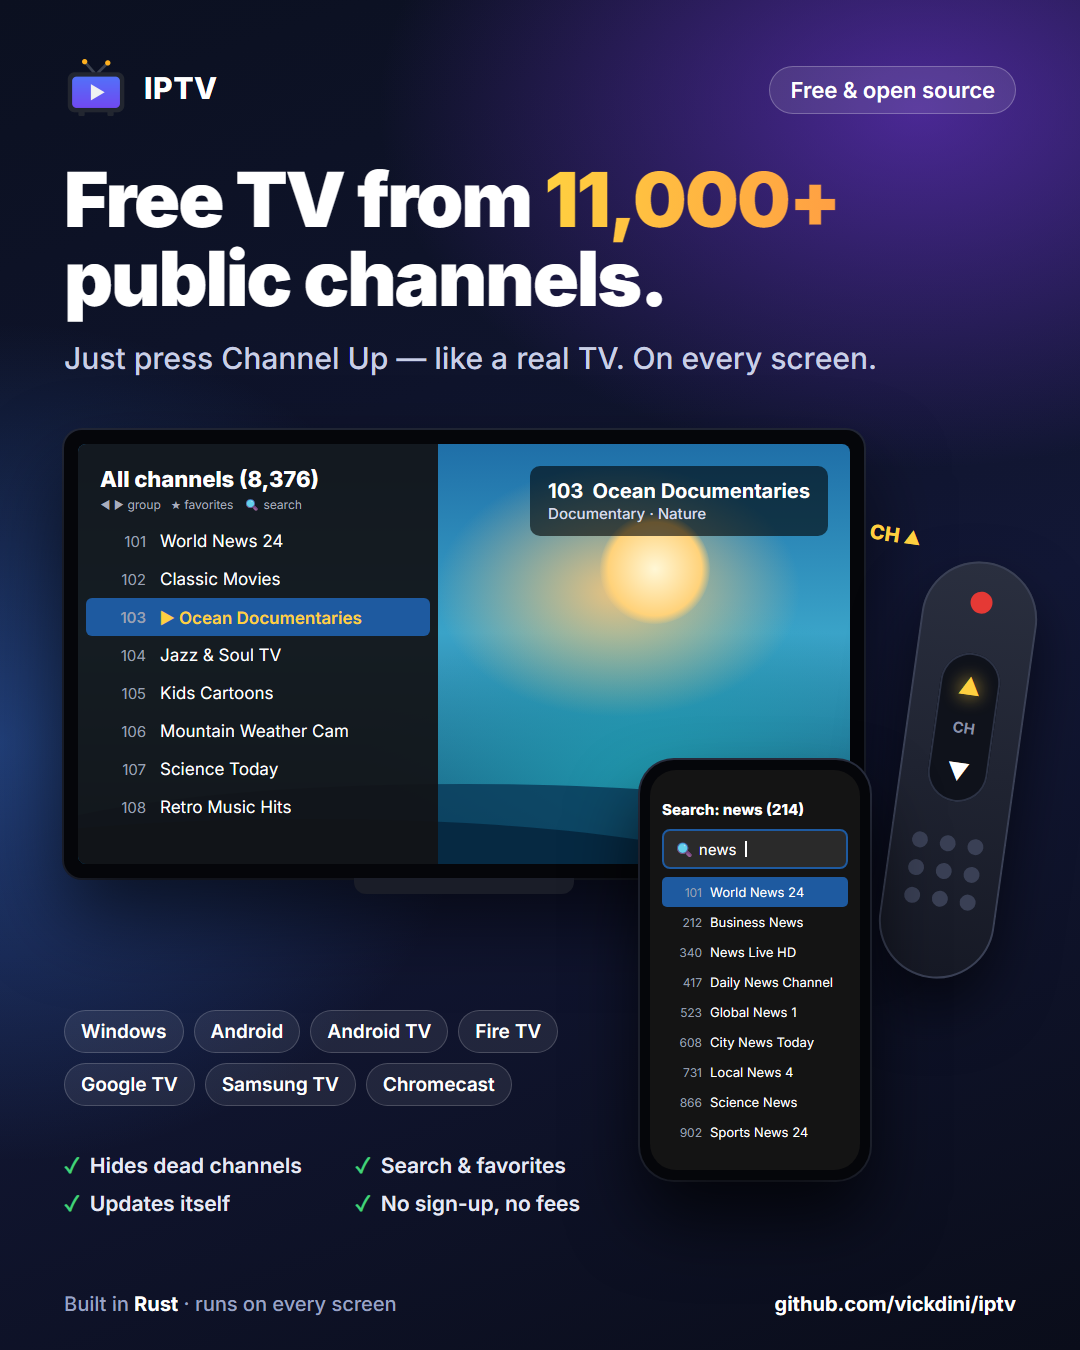
\includegraphics[width=0.52\textwidth]{../images/iptv-overview.png}\par
  \vfill
  {\large Windows \textbullet{} macOS \textbullet{} Linux \textbullet{} Android
   \textbullet{} Android TV \& Fire TV \textbullet{} Chromecast \textbullet{} Samsung TV\par}
  \vspace{0.5cm}
  {\color{dim} #2 \version{} \textbullet{} \url{https://github.com/vickdini/iptv}\par}
\end{titlepage}
\tableofcontents
\thispagestyle{fancy}}
:
%   \GuideLang   babel language (english, italian, spanish, french, ngerman, portuguese)
%   \GuideTitle  the guide's title, used on the cover, in headers and the PDF
%   \TipLabel    the word that starts a tip box ("Tip.")
% Build any of them with pdflatex, twice (for the table of contents).
\documentclass[11pt,a4paper]{article}

\usepackage[T1]{fontenc}
\usepackage[utf8]{inputenc}
% shorthands=off: no language-specific active characters (they would clash
% with tables and addresses); only hyphenation and "Contents" etc. change.
\usepackage[shorthands=off,\GuideLang]{babel}
\usepackage{lmodern}
\usepackage[scaled=0.92]{helvet}
\renewcommand{\familydefault}{\sfdefault}
\usepackage[margin=2.2cm,headheight=14pt]{geometry}
\usepackage{graphicx}
\usepackage[table]{xcolor}
\usepackage{booktabs}
\usepackage{tabularx}
\usepackage{xltabular}
\usepackage{enumitem}
\usepackage{titlesec}
\usepackage{fancyhdr}
\usepackage{pifont}
\usepackage{amssymb}
\usepackage[hidelinks]{hyperref}

\newcommand{\version}{0.12}
\definecolor{accent}{HTML}{1E6FD9}
\definecolor{dim}{HTML}{5F6673}
\definecolor{notebg}{HTML}{EEF4FC}
\definecolor{warnbg}{HTML}{FFF6E0}
\definecolor{tvred}{HTML}{D32F2F}
\definecolor{tvgreen}{HTML}{2E7D32}
\definecolor{tvyellow}{HTML}{C9A400}
\definecolor{tvblue}{HTML}{1565C0}

\hypersetup{pdftitle={IPTV -- \GuideTitle}, pdfauthor={IPTV project}}
\setlist{itemsep=2pt, topsep=4pt}
\setlength{\parindent}{0pt}
\setlength{\parskip}{6pt}
\renewcommand{\arraystretch}{1.25}

\titleformat{\section}{\Large\bfseries\color{accent}}{\thesection}{0.6em}{}
\titleformat{\subsection}{\large\bfseries}{\thesubsection}{0.6em}{}
\titlespacing*{\section}{0pt}{14pt}{6pt}
\titlespacing*{\subsection}{0pt}{10pt}{4pt}

\pagestyle{fancy}
\fancyhf{}
\fancyhead[L]{\small\color{dim}IPTV -- \GuideTitle}
\fancyhead[R]{\small\color{dim}github.com/vickdini/iptv}
\fancyfoot[C]{\small\color{dim}\thepage}
\renewcommand{\headrulewidth}{0.4pt}
\renewcommand{\sectionmark}[1]{\markboth{#1}{}}

% A key or button on a keyboard / remote.
\newcommand{\key}[1]{{\setlength{\fboxsep}{1.5pt}\fbox{\footnotesize\vphantom{Ay}#1}}}
% A coloured remote button.
\newcommand{\colorkey}[2]{\textcolor{#1}{\ding{108}}\,\textbf{#2}}
% Shaded boxes for tips and notes.
\newcommand{\tip}[1]{\par\noindent\colorbox{notebg}{\parbox{\dimexpr\linewidth-2\fboxsep}{\small\textbf{\TipLabel} #1}}\par}
\newcommand{\note}[1]{\par\noindent\colorbox{warnbg}{\parbox{\dimexpr\linewidth-2\fboxsep}{\small #1}}\par}
\newcommand{\menu}[1]{\textit{#1}}
\newcommand{\download}{\url{https://github.com/vickdini/iptv/releases/latest}}
% Key tables: \rowcolors{2}{gray!8}{white} then
% \begin{xltabular}{\linewidth}{@{}KX@{}} \keyshead{Key}{What it does} ... \bottomrule
\newcolumntype{K}{>{\raggedright\arraybackslash}p{5.4cm}}
\newcommand{\keyshead}[2]{\toprule \textbf{#1} & \textbf{#2} \\ \midrule}

% The cover: #1 subtitle, #2 "Version".
\newcommand{\cover}[2]{%
\begin{titlepage}
  \centering
  \vspace*{0.5cm}
  {\fontsize{40}{48}\selectfont\bfseries\color{accent} IPTV\par}
  \vspace{0.3cm}
  {\LARGE \GuideTitle\par}
  \vspace{0.3cm}
  {\large\color{dim} #1\par}
  \vspace{1cm}
  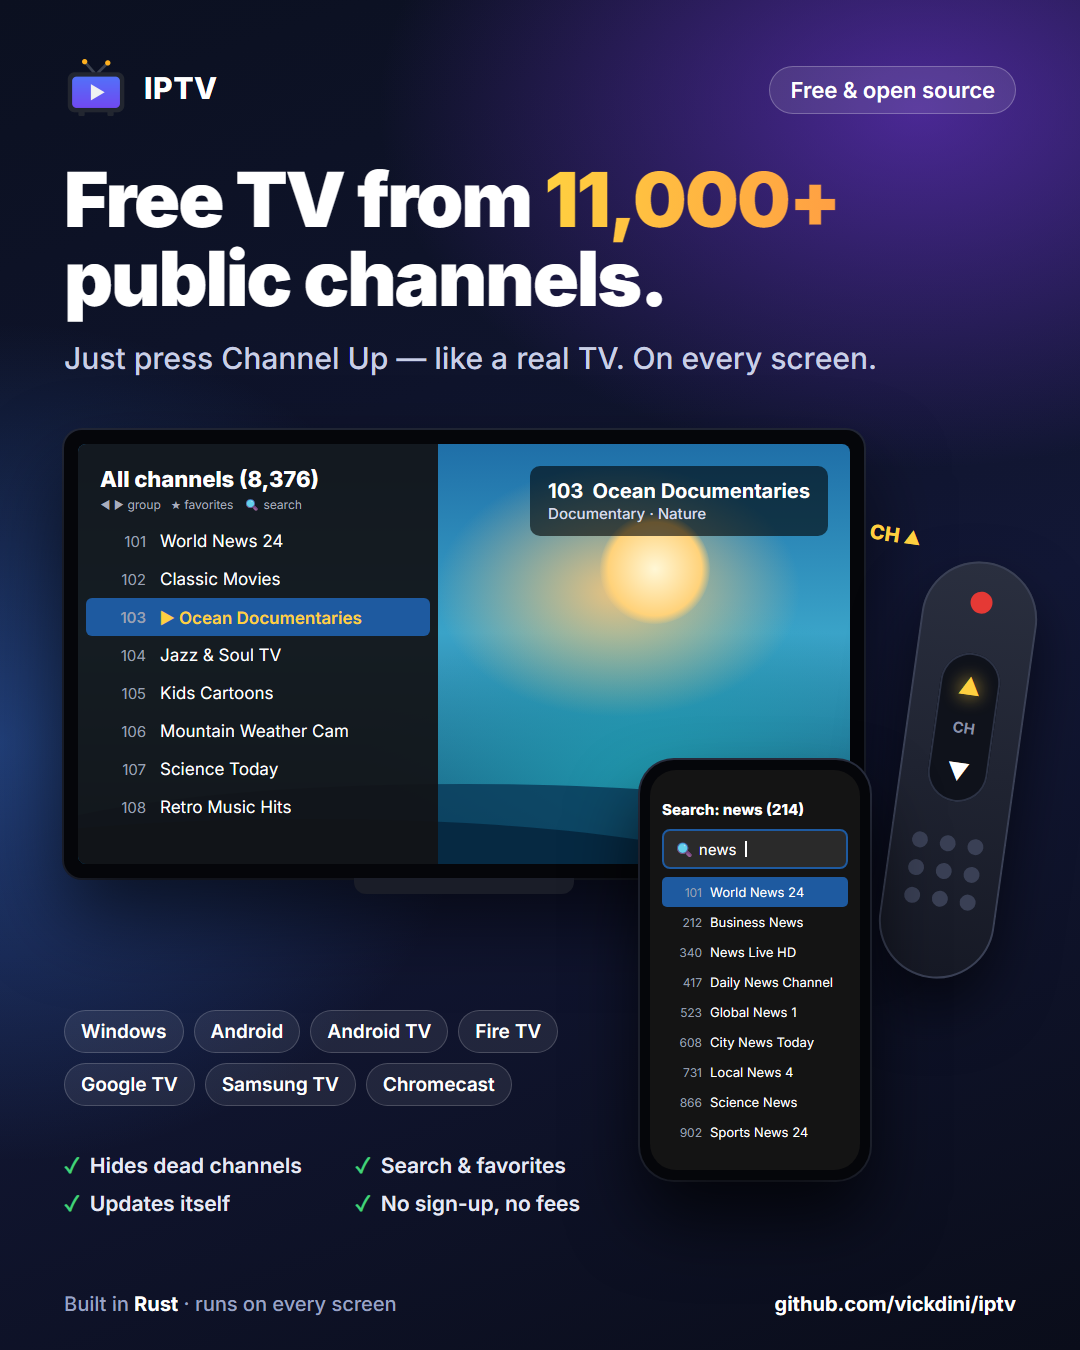
\includegraphics[width=0.52\textwidth]{../images/iptv-overview.png}\par
  \vfill
  {\large Windows \textbullet{} macOS \textbullet{} Linux \textbullet{} Android
   \textbullet{} Android TV \& Fire TV \textbullet{} Chromecast \textbullet{} Samsung TV\par}
  \vspace{0.5cm}
  {\color{dim} #2 \version{} \textbullet{} \url{https://github.com/vickdini/iptv}\par}
\end{titlepage}
\tableofcontents
\thispagestyle{fancy}}
